\documentclass[../differential_geometry.tex]{subfiles}
\begin{document}
\section{Aula 17 - 02 de Junho, 2026}
\subsection{Motivações}
\begin{itemize}
	\item A Curvatura Normal.
\end{itemize}
\subsection{A Curvatura Normal}
\begin{def*}
	O coeficiente \(\kappa_{n}\) é a \textbf{curvatura normal de \(\mathbf{\beta }\)}, e \(\kappa_{g}(s)\) é a \textbf{curvatura geodésica de \(\mathbf{\beta }\)}. \(\square\)
\end{def*}
\begin{figure}[H]
	\begin{center}
		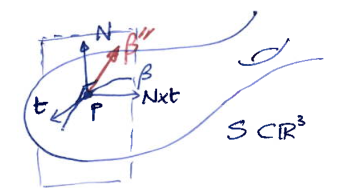
\includegraphics[height=0.5\textheight, width=0.5\textwidth, keepaspectratio]{./Images/normal_curvature_17.png}
	\end{center}
\end{figure}
Considerando \(\beta \) como uma curva em \(\mathbb{R}^{3}\), temos \(\beta ''= \kappa n\), tal que
\[
	\kappa n = \kappa_{g} N\times t + \kappa_{n}N,
\]
e por \(n, N\times t\) e N serem todo unitários, além de \(\langle N\times t, N \rangle = 0\), obtemos
\[
	\boxed{\kappa^{2} = \kappa_{g}^{2} + \kappa_{n}^{2}}
\]
Vamos supor, agora, que \(\beta \) é a curva obtida pela interseção da superfície S com um plano passando por p em S e gerado por \(N(p)\), e que \(w\in T_pS\) com w unitário. Neste caso, \(\beta''\) é paralelo a N, e portanto
\[
	\kappa_{g} = 0 \Rightarrow \kappa = \pm \kappa_{n}.
\]
\begin{figure}[H]
	\begin{center}
		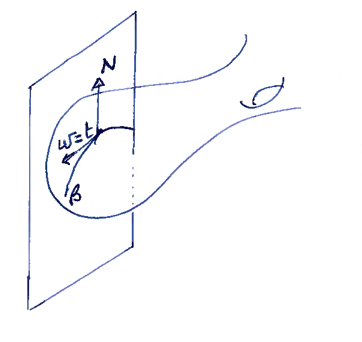
\includegraphics[height=0.7\textheight, width=0.7\textwidth, keepaspectratio]{./Images/observation_17.png}
	\end{center}
\end{figure}
Vamos calcular \(\kappa_{n}\); temos \(\beta''=\kappa_{g}N\times t + \kappa_{n}N\), e fazendo o produto escalar com N, obtemos
\[
	\langle \beta '', N \rangle = \langle \kappa_{g}N\times t + \kappa_{n}, N \rangle,
\]
mas com \(\langle \beta ', N \rangle \) identicamente nulo, segue que
\[
	\langle \beta '', N \rangle + \langle \beta ', N' \rangle = 0,
\]
ou seja,
\[
	\langle \beta'', N \rangle=-\langle N', \beta ' \rangle = \langle -\mathrm{d}N_{p}(\beta'), \beta'  \rangle = \mathbb{I}_{p}(\beta'),
\]
Portanto, quando \(\beta \) é parametrizada por comprimento de arco, a curvatura normal coincide com a segunda forma fundamental de \(\beta \) calculada no ponto \(p = \beta (s)\).

\begin{tcolorbox}[
		skin=enhanced,
		title=Observação,
		fonttitle=\bfseries,
		colframe=black,
		colbacktitle=cyan!75!white,
		colback=cyan!15,
		colbacklower=black,
		coltitle=black,
		drop fuzzy shadow,
		%drop large lifted shadow
	]
	A curvatura normal de \(\beta \) em \(\beta (s)\) depende somente do vetor tangente unitário \(\beta '(s)\) em \(\beta (s)\), não da curva \(\beta \).
\end{tcolorbox}

Por outro lado, se \(\beta \) não for parametrizada por comprimento de arco, teremos
\[
	\kappa_{n}=\mathbb{I}_{p}\biggl(\frac{\beta '}{\Vert \beta ' \Vert}\biggr) = \biggl\langle -\mathrm{d}N_{p}\biggl(\frac{\beta '}{\Vert \beta ' \Vert}\biggr), \frac{\beta '}{\Vert \beta ' \Vert} \biggr\rangle = \frac{1}{\Vert \beta'  \Vert^{2}}\langle -\mathrm{d}N_{p}(\beta '), \beta ' \rangle,
\]
isto é, a curvatura normal é dada pela razão da segunda forma fundamental pela primeira da curva \(\beta '\):
\[
	\boxed{\kappa_{n}= \frac{\mathbb{I}_{p}(\beta ')}{I_{p}(\beta ')}}
\]

Se \(\underline{x}:U\rightarrow S \subseteq \mathbb{R}^{3}\) for uma parametrização local de S e \(\beta '=a \underline{x}_{n} + b \underline{x}_{v}\in T_{p}S,\) com \(p = \beta (s)\), temos a forma explícita
\[
	\boxed{\kappa_{n} = \frac{a^{2}\ell +2ab m + b^{2}n}{a^{2}E+2abF+b^{2}G}}
\]

\hypertarget{meusnier_theorem}{
	\begin{theorem*}[Meusnier]
		Todas as curvas sobre um superfície \(S\subseteq \mathbb{R}^{3}\) que passam por um ponto p de S e que têm a mesma reta tangente em p, tem a mesma curvatura normal em p dada por \(\mathbb{I}_{p}(t)\), onde t é um vetor tangente unitário das curvas no ponto p.
	\end{theorem*}
}
\begin{def*}
	Seja e um vetor unitário de \(T_{p}S\); chamamos \(\kappa_{n} = \mathbb{I}_{p}(e)\) de \textbf{curvatura normal de S no ponto p, ao longo da direção e}. \(\square\)
\end{def*}

\begin{example}
	Vamos considerar a parametrização local
	\[
		\underline{x}(u, v) = \biggl(u, v, \frac{1}{2}(u^{2}-v^{2})\biggr).
	\]
	Pelas contas que fizemos outrora, no ponto \(p = \underline{x}(0, 0) = (0, 0, 0)\), temos
	\[
		E = 1, \quad F = 0, \quad G = 1, \quad \ell =1, \quad m=0 \quad\&\quad n = -1,
	\]
	e
	\[
		\underline{x}_{u}=(1, 0, 0), \quad \underline{x}_{v} = (0, 1, 0) \quad\&\quad  N = (0, 0, 1).
	\]
	A matriz de \(\mathrm{d}N_{p}\) em relação à base \(\{\underline{x}_{u}, \underline{x}_{v}\}\) de \(T_{p}S\) é dada por
	\[
		-\mathrm{d}N_{p} = \frac{1}{EG - F^{2}}\begin{bmatrix}
			G  & -F \\
			-F & E
		\end{bmatrix} \begin{bmatrix}
			\ell & m \\
			m    & n
		\end{bmatrix} = \begin{bmatrix}
			1 & 0  \\
			0 & -1
		\end{bmatrix}.
	\]
	Logo, \(\underline{x}_{u}\) e \(\underline{x}_{v}\) são autovetores no ponto p com autovalores \(\kappa_{2} = 1\) e \(\kappa_{1}=-1\); qualquer vetor unitário \(e\in T_{p}S\) pode ser tomado na forma
	\[
		e(\theta ) = \cos^{}{(\theta)}\underline{x}_{u} + \sin^{}{(\theta)}\underline{x}_{v}.
	\]
	Portanto,
	\[
		\kappa_{n}(\theta ) = \kappa_{n}(e(\theta )) = \mathbb{I}_{p}(e(\theta ))=\cos^{2}{\theta }-\sin^{2}{\theta } = \cos^{}{2\theta }.
	\]
	Podemos tirar disso que
	\[
		\kappa_{1}=-1 \leq \kappa_{n}(\theta ) \leq \kappa_{2}=1,
	\]
	e, mais ainda,
	\begin{align*}
		\kappa_{n}'(\theta ) = -2\sin^{}{2\theta } & =0                                                                      \\
		\Longleftrightarrow                        & \theta  = 0 \text{ ou }\frac{\varphi }{2}                               \\
		\Longleftrightarrow                        & e(\theta ) = \underline{x}_{u} \text{ ou } e(\theta )=\underline{x}_{v}
	\end{align*}
\end{example}
\begin{prop*}
	Seja \(p\in S\subseteq \mathbb{R}^{3}\) um ponto não umbílico (\(\kappa_1\neq \kappa_2\)). Então, o máximo e o mínimo da curvatura normal \(\kappa_{n}(e)\) quando \(e\) varia no círculo unitário em \(T_{p}S\) são as curvaturas principais \(\kappa_2\) e \(\kappa_1\), correspondendo às direções principais associadas a cada uma delas.
\end{prop*}
\begin{proof*}
	Como \(\kappa_1\neq \kappa_2\), existem dois autovetores ortogonais \(e_1\) e \(e_2\) de \(-\mathrm{d}N_{p}\) em \(T_{p}S\):
	\begin{align*}
		 & -\mathrm{d}N_{p}(e_1) = \kappa_1e_1  \\
		 & -\mathrm{d}N_{p}(e_2) = \kappa_2e_2,
	\end{align*}
	tal que, tomando \(e(\theta ) = \cos^{}{\theta }e_1 + \sin^{}{\theta }e_2\in T_{p}S\) unitário, obtemos:
	\begin{align*}
		\kappa_{n}(\theta ) = \kappa_{n}(e(\theta )) & =\mathbb{I}_{p}(e(\theta ))                                                                                             \\
		                                             & =\langle -\mathrm{d}N_{p}(\cos^{}{\theta }e_1 + \sin^{}{\theta }e_2), \cos^{}{\theta }e_1 + \sin^{}{\theta }e_2 \rangle \\
		                                             & = \langle \kappa_1\cos^{}{\theta }e_1 + \kappa_2\sin^{}{\theta }e_2, \cos^{}{\theta }e_1 + \sin^{}{\theta }e_2 \rangle  \\
		                                             & = \kappa_1\cos^{2}{\theta } + \kappa_2 \sin^{2}{\theta }.
	\end{align*}
	Derivando com respeito a \(\theta \),
	\[
		\kappa_{n}'(\theta ) = (\kappa_2-\kappa_1)\sin^{}{2\theta };
	\]
	logo,
	\[
		\kappa_{n}'(\theta )=0\Longleftrightarrow \theta =0 \text{ ou }\frac{\pi }{2}.
	\]
	Para \(\theta =0\), teremos \(e(0)=e_1\) e \(\kappa_{n}(0) = \kappa_1\); para \(\displaystyle \theta = \frac{\pi }{2}\), vale
	\[
		e\biggl(\frac{\pi }{2}\biggr) = e_2 \quad\&\quad \kappa_{n}\biggl(\frac{\pi }{2}\biggr)=\kappa_2.
	\]
	Portanto, assumindo (sem perda de generalidade) \(\kappa_1 < \kappa_2\)
	\[
		\kappa_1 \leq \kappa_{n}(\theta ) \leq \kappa_2. \text{ \qedsymbol}
	\]
\end{proof*}
\begin{exr}
	Seja S uma superfície em \(\mathbb{R}^{3}\) e \(\kappa_{n}(\theta )\) a curvatura normal de S em \(p\in T_pS\) ao longo do vetor \(e(\theta ) = \cos^{}{\theta }e_1+\sin^{}{\theta }e_2\). Calcule
	\[
		\frac{1}{2\pi }\int_{0}^{2\pi }\kappa_{n}(\theta ) \mathrm{d}\theta .
	\]

	\textbf{\underline{Solução}}: basta fazer as contas
	\begin{align*}
		\frac{1}{2\pi }\int_{0}^{2\pi }\kappa_{n}(\theta ) \mathrm{d}\theta & =\frac{1}{2\pi }\int_{0}^{2\pi }(\kappa_1\cos^{2}{\theta } + \kappa_2\sin^{2}{\theta }) \mathrm{d}\theta                                                                              \\
		                                                                    & =\frac{1}{2\pi }\biggl(\frac{1}{2}(\theta +\sin^{}{\theta }\cos^{}{\theta })\kappa_1 + \frac{1}{2}(\theta -\sin^{}{\theta }\cos^{}{\theta })\kappa_2\biggr)\biggl|_{0}^{2\pi }\biggr. \\
		                                                                    & =\frac{1}{2\pi }(\pi \kappa_1 + \pi \kappa_2)                                                                                                                                         \\
		                                                                    & =\frac{1}{2}(\kappa_1+\kappa_2)                                                                                                                                                       \\
		                                                                    & = H,
	\end{align*}
	que é a curvatura média.
\end{exr}
\subsection{Classificação de Pontos em Superfícies}
\begin{def*}
	Seja S uma superfície em \(\mathbb{R}^{3}\). Um ponto p em S é:
	\begin{itemize}
		\item \textbf{elíptico} se \(\kappa (p) > 0\);
		\item \textbf{hiperbólico} se \(\kappa(p) < 0\);
		\item \textbf{parabólico} se \(\kappa(p) = 0.\; \square\)
	\end{itemize}
\end{def*}
Vimos que \(\kappa_{n}(\theta )\) depende somente da direção determinada por \(\theta \in S^{1}\subseteq T_{p}S\) e não da curva \(\beta \subseteq S\) com \(\beta(0) = p\) e \(\beta '(0) = \cos^{}{\theta }e_1 + \sin^{}{\theta }e_2\).
Podemos escolher \(\beta \) como sendo a curva plana obtida pela interseção de S com o plano por p e paralelo a \(N(p)\) e \(\beta '(0)\); chmamos tal curva de \textbf{seção normal}.

\textbf{\textit{Em um ponto elíptico}}, \(\kappa (p) = \kappa_1\kappa_2 > 0\), permitindo concluir que \(\kappa_1\) e \(\kappa_2\) têm o mesmo sinal; como \(\kappa_1 \leq \kappa_{n}(\theta )\leq \kappa_2\), segue que todas as curvas normais \(\kappa_{n}(\theta )\) têm o mesmo sinal, ou seja, todas as sessões normais de S em p têm o mesmo sinal para suas curvaturas! Por isso, a superfície tem localmente a seguinte forma:
\begin{figure}[H]
	\begin{center}
		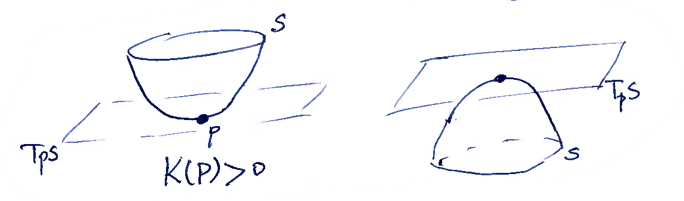
\includegraphics[height=\textheight, width=\textwidth, keepaspectratio]{./Images/elliptical_point_17.png}
	\end{center}
\end{figure}

\textbf{\textit{Em um ponto hiperbólico}}, \(\kappa_1\) e \(\kappa_2\) têm sinais opostos; então, existem seções normais com curvatura positiva e outras com curvaturas negativas, dando a forma local de uma sela:
\begin{figure}[H]
	\begin{center}
		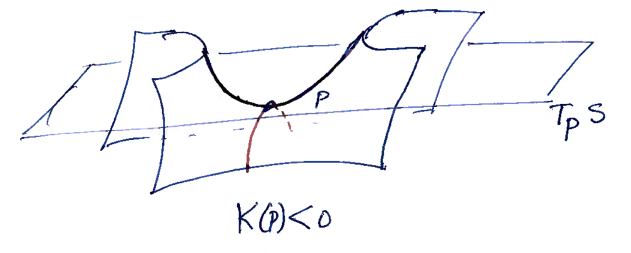
\includegraphics[height=\textheight, width=\textwidth, keepaspectratio]{./Images/hyperbolic_point_17.png}
	\end{center}
\end{figure}

\textbf{\textit{Nos pontos parabólicos}}, por sua vez, a curva separa uma região elíptica e a região hiperbólica da superfície:
\begin{figure}[H]
	\begin{center}
		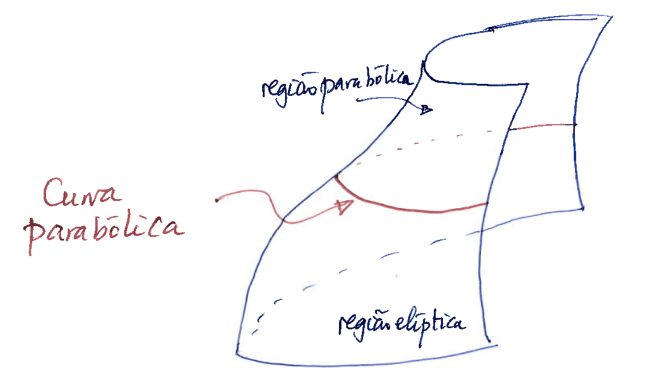
\includegraphics[height=\textheight, width=\textwidth, keepaspectratio]{./Images/parabollic_curve_17.png}
	\end{center}
	\caption{Nestas regiões, é possível apoiar a superfície em cima de um plano! Tente determinar os pontos parabólicos de uma laranja.}
\end{figure}

\subsection{Direções Assintóticas}
\begin{def*}
	Uma direção em \(T_{p}S\) representada por \(\theta \in S^{1}\subseteq T_{p}S\) é chamada \textbf{direção assintótica} se \(\kappa_{n}(\theta ) = 0.\; \square\)
\end{def*}
Se p é um ponto elíptico, \(\kappa_{n}(\theta ) > 0\) ou \(\kappa_{n}(\theta ) < 0\) para todo \(\theta \), significando que não existem direções assintóticas em \(T_{p}S\); por outro lado, se p é um ponto hiperbólico, então
\begin{align*}
	\kappa_{n} (\theta ) = \kappa_1\cos^{2}{\theta}+\kappa_2\sin^{2}{\theta } & =0                                                      \\
	\Longleftrightarrow                                                       & \tan^{2}{\theta } = -\frac{\kappa_1(p)}{\kappa_2(p)}    \\
	\Longleftrightarrow                                                       & \tan^{}{t} = \sqrt[]{-\frac{\kappa_1(p)}{\kappa_2(p)}},
\end{align*}
garantindo a existência de duas direções assintóticas em cada ponto hiperbólico:
\begin{figure}[H]
	\begin{center}
		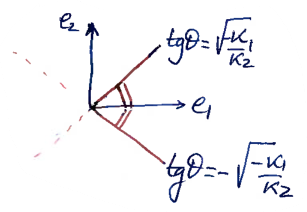
\includegraphics[height=0.8\textheight, width=0.8\textwidth, keepaspectratio]{./Images/asymptotic_directions_17.png}
	\end{center}
\end{figure}
\subsection{Famílias de Curvas em Superfícies}
\begin{def*}
	Uma curva \(\beta (t)\subseteq S\) é uma \textbf{linha de curvatura} se \(\beta '(t)\) é sempre na direção de uma direção principal.
\end{def*}
Por cada ponto não umbílico (\(\kappa_1\neq \kappa_2\)), passam duas linhas de curvatura que se intersectam ortogonalmente no ponto.

\begin{example}
	Seja S o gráfico de \(z=\frac{1}{2}(x^{2}-y^{2})\), parametrizada por
	\[
		\underline{x}(u, v) = (u+v, u-v, 2uv).
	\]
	Temos:
	\[
		\underline{x}_{u}=(1, 1, 2v),\; \underline{x}_{v}(1, -1, 2u),\; \underline{x}_{uu}=(0, 0, 0),\; \underline{x}_{uv}=(0, 0, 2) \;\&\; \underline{x}_{vv}=(0, 0, 0).
	\]
	Assim,
	\[
		N = \frac{(u+v, v-u, -1)}{\sqrt[]{1+u^{2}+v^{2}}},
	\]
	e portanto
	\begin{align*}
		 & E = 2 + 4v^{2},\quad\ell =0                        \\
		 & F = 4uv,\quad m =-\frac{2}{\sqrt[]{1+u^{2}+v^{2}}} \\
		 & E = 2 + 4u^{2},\quad n =0.
	\end{align*}
	Com esta descrição, podemos determinar que uma direção \(a\underline{x}_u + b\underline{x}_v\) é assintótica se, e somente se,
	\[
		\det \begin{bmatrix}
			b^{2} & -ab & a^{2} \\
			E     & F   & G     \\
			\ell  & m   & n
		\end{bmatrix} = 0 \Longleftrightarrow \det \begin{bmatrix}
			b^{2}    & -ab & a^{2}    \\
			1+2v^{2} & 2uv & 1+2u^{2} \\
			0        & 1   & 0
		\end{bmatrix} = 0,
	\]
	que equivale a
	\[
		(-1+2u^{2})b^{2} = (1+2v^{2})a^{2} \Longleftrightarrow \sqrt[]{1+2u^{2}}b = \pm \sqrt[]{1+2v^{2}}a.
	\]
	Logo, se \(\beta (t)=\underline{x}(u(t), v(t))\) é uma linha de curvatura, então \(\beta' =u'\underline{x}_u + v'\underline{x}_v\) é uma direção principal. Logo,
	\begin{align*}
		                    & \sqrt[]{1+2u^{2}}v'=\pm \sqrt[]{1+2v^{2}}u'                                                                 \\
		\Longleftrightarrow & \frac{u'}{\sqrt[]{1+2u^{2}}} = \pm \frac{v'}{\sqrt[]{1+2v^{2}}}                                             \\
		\Rightarrow         & \int_{}^{}\frac{u'}{\sqrt[]{1+2u^{2}}} \mathrm{d}t = \pm \int_{}^{}\frac{v'}{\sqrt[]{1+2v^{2}}} \mathrm{d}t \\
		\Longleftrightarrow & \mathrm{arcsinh}(\sqrt[]{2}u) = \pm \mathrm{arcsinh}(\sqrt[]{2}v)+c.
	\end{align*}
	Com isso, as famílias de curvas em \(U\subseteq \mathbb{R}^{2}\), dadas, para algum c em \(\mathbb{R}\), por
	\begin{align*}
		 & \mathrm{arcsinh}(\sqrt[]{2}u) + \mathrm{arcsinh}(\sqrt[]{2}v) = c  \\
		 & \mathrm{arcsinh}(\sqrt[]{2}u) - \mathrm{arcsinh}(\sqrt[]{2}v) = c,
	\end{align*}
	parametrizam as linhas de curvatura em S.
	\begin{figure}[H]
		\begin{center}
			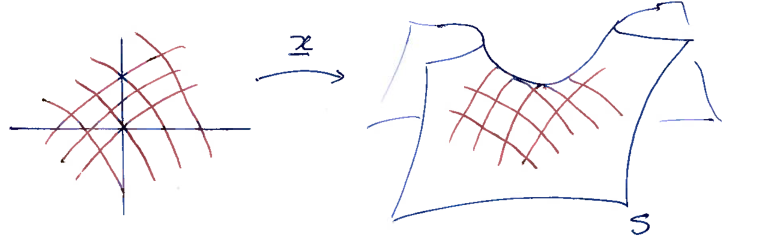
\includegraphics[height=\textheight, width=\textwidth, keepaspectratio]{./Images/asin_curvature_18.png}
		\end{center}
	\end{figure}
\end{example}
\begin{example}[Superfícies de Revolução]
	Seja \(\underline{x}(u, v) = (f(v)\cos^{}{u}, f(v)\sin^{}{u}, g(v))\) uma parametrização local da superfície de revolução obtida girando a curva
	\[
		\alpha (v) = (f(v), 0, g(v))
	\]
	em torno do eixo z. Temos:
	\begin{align*}
		 & \underline{x}_{u} = (-f(v)\sin^{}{u}, f(v)\cos^{}{u}, 0),                                                                                                                                       \\
		 & \underline{x}_{v} = (f'(v)\cos^{}{u}, f'(v)\sin^{}{u}, g'(v)),                                                                                                                                  \\
		 & \underline{x}_{uu} = (-f(v)\cos^{}{u}, -f(v)\sin^{}{u}, 0),                                                                                                                                     \\
		 & \underline{x}_{uv} = (-f'(v)\sin^{}{u}, f'(v)\cos^{}{u}, 0),                                                                                                                                    \\
		 & \underline{x}_{vv} = (f''(v)\cos^{}{u}, f''(v)\sin^{}{u}, g''(v)),                                                                                                                              \\
		 & N = \frac{\underline{x}_{u}\times \underline{x}_{v}}{\Vert \underline{x}_u \times \underline{x}_v \Vert} = \frac{(g'(v)\cos^{}{u}, g'(v)\sin^{}{u}, -f'(v))}{\sqrt[]{(f')^{2}(v)+(g')^{2}(v)}}.
	\end{align*}
	Daí,
	\begin{align*}
		 & E = f^{2}(v), \quad \ell = - \frac{f(v)g'(v)}{\sqrt[]{(f')^{2}(v) + (g')^{2}(v)}}                                  \\
		 & F = 0, \quad m = 0                                                                                                 \\
		 & G = (f')^{2}(v) + (g')^{2}(v) \quad\&\quad n = \frac{f''(v)g'(v)-f'(v)g''(v)}{\sqrt[]{(f')^{2}(v) + (g')^{2}(v)}}.
	\end{align*}
	Uma direção \(a\underline{x}_u + b\underline{x}_v\) é principal se, e somente se,
	\[
		\det \begin{bmatrix}
			b^{2} & -ab & a^{2} \\
			E     & 0   & G     \\
			\ell  & 0   & n
		\end{bmatrix} = 0 \Longleftrightarrow (En - \ell G)ab = 0.
	\]
	Nos pontos onde \(En-\ell G \neq 0\), as soluções são \(a=0\) ou \(b=0\), ou seja, são \(\underline{x}_{u}\) e \(\underline{x}_v\). Portanto, as linhas de curvatura são as paralelas às meridianas.
\end{example}
\end{document}

